\documentclass[onecolumn]{article}
%\usepackage{url}
%\usepackage{algorithmic}
\usepackage[utf8]{inputenc}
\usepackage[a4paper]{geometry}
\usepackage[nodayofweek]{datetime}
\newcommand{\mydate}{\formatdate{20}{01}{2022}}
\usepackage{booktabs}
\usepackage{tabu}
\usepackage[margin=2em, font=small,labelfont=it,bf]{caption}
\usepackage{graphicx}
\usepackage{fancyhdr}
\usepackage{mathpazo} % use palatino
\usepackage[scaled]{helvet} % helvetica
\usepackage{microtype}
\usepackage{amsmath}
\usepackage{subfigure}
\usepackage[style=chem-acs, articletitle=true]{biblatex}
\addbibresource{references.bib}

\usepackage{hyperref}

\setlength{\parskip}{1em}
\setlength{\parindent}{0em}

% Letterspacing macros
\newcommand{\spacecaps}[1]{\textls[200]{\MakeUppercase{#1}}}
\newcommand{\spacesc}[1]{\textls[50]{\textsc{\MakeLowercase{#1}}}}


\title{\spacecaps{Characterise gene expression differences
between human breast cancer subtypes }\\ \normalsize \spacesc{467713-HS2021, RNA-sequencing} }

\author{Shunyu Wu\\shunyu.wu@students.unibe.ch \\  github.com/kitamado/DE-analysis  \\}



%\date{\today\\\currenttime}
\date{\mydate}

\begin{document}
\maketitle

\rule{\textwidth}{0.1pt}
\begin{abstract}
The purpose of this project is to generate lists of genes that differ in expression across two experimental groups and to discover gene ontology (GO) concepts that are enriched for DE genes. To do this, I Assessed the read number and quality, mapped the reads to the human reference genome GRCh38 and then counted the number of reads overlapping annotated genes. The counts were used to perform a differential expression and a overrepresentation analysis. Many of the primary GO terms discovered are related to the immune system.
\end{abstract}
\rule{\textwidth}{0.1pt}

\section{Introduction}
Breast cancer is the most common cause of cancer mortality in women, it lacks a well defined genetic landscape so the main treatment challenge is to recognize the precise forms of disease and the biology that underpins them. By massively parallel mRNA sequencing, Eswaran et al\cite{Eswaran2012} gathered 1.2 billion reads from 17 unique human tissues. The workflow from raw sequence reads to DE analysis includes RNA extraction and library preparation, Sequencing, quality control of raw sequencing data (FastQC), quantify expression, quality control of aligned sequence reads and aggregating results with MultiQC, generate raw counts and model to each gene, testing for differential expression and shrinking log2 fold changes.

Our data contains 3 samples each from normal breast tissue and 3 different breast cancer subtypes: \emph{Triple negative, HER2 positive, Non-triple negative (Luminal A/B)}.
 I use HiSat2 algorithm and Samtools to map those human breast cancer sample RNA-seq reads to human reference genome (GRCh38). Then I choose featureCounts tool to start with a matrix of counts representing the levels of gene expression in order to perform Differential Gene Expression analysis.


\section{Data sets}

The data utilized is a subset of Eswaran et al\cite{Eswaran2012}, consisting of fastq files obtained from the Gene Expression Omnibus (GEO), accession GSE52194. The libraries were sequenced in paired-end mode on an Illumina HiSeq 2000, 2 files per sample, for read 1 and read 2 respectively. There are 4 experimental groups with 3 replicates each, every sample has 2 reads. Library prep protocol did not preserve information on the transcribed strand(non-stranded). 
\begin{itemize}
   \item Normal: Healthy controls
    \item TNBC: Triple negative breast cancer
    \item NonTNBC: Non triple negative breast cancer
   \item HER2: HER2 positive breast cancer
\end{itemize}

 The reference genome (assembly GRCh38) \verb|Homo_sapiens.GRCh38.dna.primary_assembly.fa.gz|  and associated annotation \verb|Homo_sapiens.GRCh38.104.gtf.gz| were download from the Ensembl ftp site. 

\section{Methods and Results}
\subsection{Quality checks}

MultiQC(v.1.8)\cite{10.1093/bioinformatics/btw354} was used to summarize the FastQC(v.0.11.7)\cite{FastQC} reports, together used to evaluate the subset's quality.

\begin{figure}[t]
\centering
\subfigure[Sequence Counts]{\centering
    \includegraphics[width=.4\linewidth]{fig/fastqc_sequence_counts_plot.png}
        \label{fig:sequence-counts}}
\subfigure[Per Sequence Quality Scores]{\centering
    \includegraphics[width=.4\linewidth]{fig/fastqc_per_base_sequence_quality_plot.png}
        \label{fig:per-base}}
\caption{\label{fig:multiQC}
Result from MultiQC output showing sequence counts for each sample (left) and the mean quality value across each base position in the read (right).}
\end{figure}


We can see from the Figure~\ref{fig:sequence-counts} and Figure~\ref{fig:per-base} that the reads number and most average base quality are good, except for HER22 reads 2. They tend to decrease a little near the end of the reads. Mate1 are usually better than mate2. Base quality decrease as reads get longer due to a unwanted but unavoidable process called phasing which limits the length of high quality reads. New chemicals are largely intended to minimize the phasing problem, increasing the length of reads before quality begins to decrease.

There might be some primer/adapter or bacterial contamination showing from the multiple peaks produced in the GC plot of FastQC html files(not attached here, see github /QCres directory). If possible we need to further processe the raw reads, using software like Trimmomatic.
 
\subsection{Map reads to the reference genome }
 Hisat2(v.2.2.1)\cite{Kim2015} was used to index and map human breast cancer RNA-seq read to human reference genome. The generated sam files were then converted to bam format, sorted and indexed using SAMtools(v.1.10)\cite{10.1093/bioinformatics/btp352}. 
 
 \begin{table}[ht!]
    \centering
    \caption{Alignment rates(\%) observed across samples. 
    }
    \begin{tabu}{*{6}{X[c]}}
        \toprule
         \textbf{HER21} & \textbf{HER22} & \textbf{HER23} & \textbf{NonTNBC1} & \textbf{NonTNBC2} & \textbf{NonTNBC3} \\
         \midrule
         91.13 & 90.63 & 94.22 & 88.86 & 88.50 & 88.09 \\
         \toprule
         \textbf{Normal1} & \textbf{Normal2} & \textbf{Normal3} & \textbf{TNBC1} & \textbf{TNBC2} & \textbf{TNBC3} \\
         \midrule
         96.51 & 96.21 & 96.58 & 89.77 & 86.69 & 85.99 \\
         \bottomrule
    \end{tabu}
    \label{tab:align-rates}
\end{table}

The original data for Table~\ref{tab:align-rates} located in \url{https://github.com/kitamado/DE-analysis/blob/main/bam/error_hisat2align_7412138.e}. We can also calculate concordant alignment, for instance, the concordant alignment for HER21 is 52101964: 25193234 (41.13\%) aligned concordantly exactly 1 time + 26908730 (43.93\%) aligned concordantly $>$ 1 times. For those with a low percentage of exactly once
concordant alignment, it is a strong evidence of multimapped reads.

 \subsection{Count the number of reads per gene}
 Finally we use featureCounts\cite{10.1093/bioinformatics/btt656}, the bam files, and the annotation file, to generate a table of counts representing the number of reads per gene.
 
  \begin{table}[ht!]
    \centering
    \caption{Reads unassigned due to Ambiguity
    }
    \begin{tabu}{*{6}{X[c]}}
        \toprule
         \textbf{HER21} & \textbf{HER22} & \textbf{HER23} & \textbf{NonTNBC1} & \textbf{NonTNBC2} & \textbf{NonTNBC3} \\
         \midrule
         2865649 & 3336145 & 2938393 & 5989589 & 2964881 & 2980577 \\
         \toprule
         \textbf{Normal1} & \textbf{Normal2} & \textbf{Normal3} & \textbf{TNBC1} & \textbf{TNBC2} & \textbf{TNBC3} \\
         \midrule
         2498473 & 4318385 & 4845160 & 2247703 & 2206447 & 2063103 \\
         \bottomrule
    \end{tabu}
    \label{tab:Unassigned_Ambiguity}
\end{table}
 
 From Table~\ref{tab:Unassigned_Ambiguity} we know the reads unassigned due to ambiguity on each group(raw data in \verb|featurecounts.txt.summary|), but keep in mind that reads align within a region corresponding to overlapping genes cannot be unambiguously assigned to either gene (e.g., the portion of the brown and yellow genes that overlap). 

\subsection{Differential expression analysis}

Whole R workflows published here: \url{https://rpubs.com/sywu/DESeq2}.

I loaded the count file in R(v.4.1.2)\cite{R} to study differential expression of genes in the three breast cancer sub-types with R package called DeSeq2(v.1.34.0)\cite{Love2014}.

 After remove the dependence of the variance on the mean by running \verb|DESeq2::rlog()|, we can generate a PCA plot Figure~\ref{fig:PCA} using the 500 most variably expressed genes. It indicates that samples from the same experimental group show similar expression patterns(can also be be conclude from the heatmap uploaded to git repo). The differential expression results were then extracted
using \verb|DESeq2::results|. 

\begin{figure}[t]
\centering
    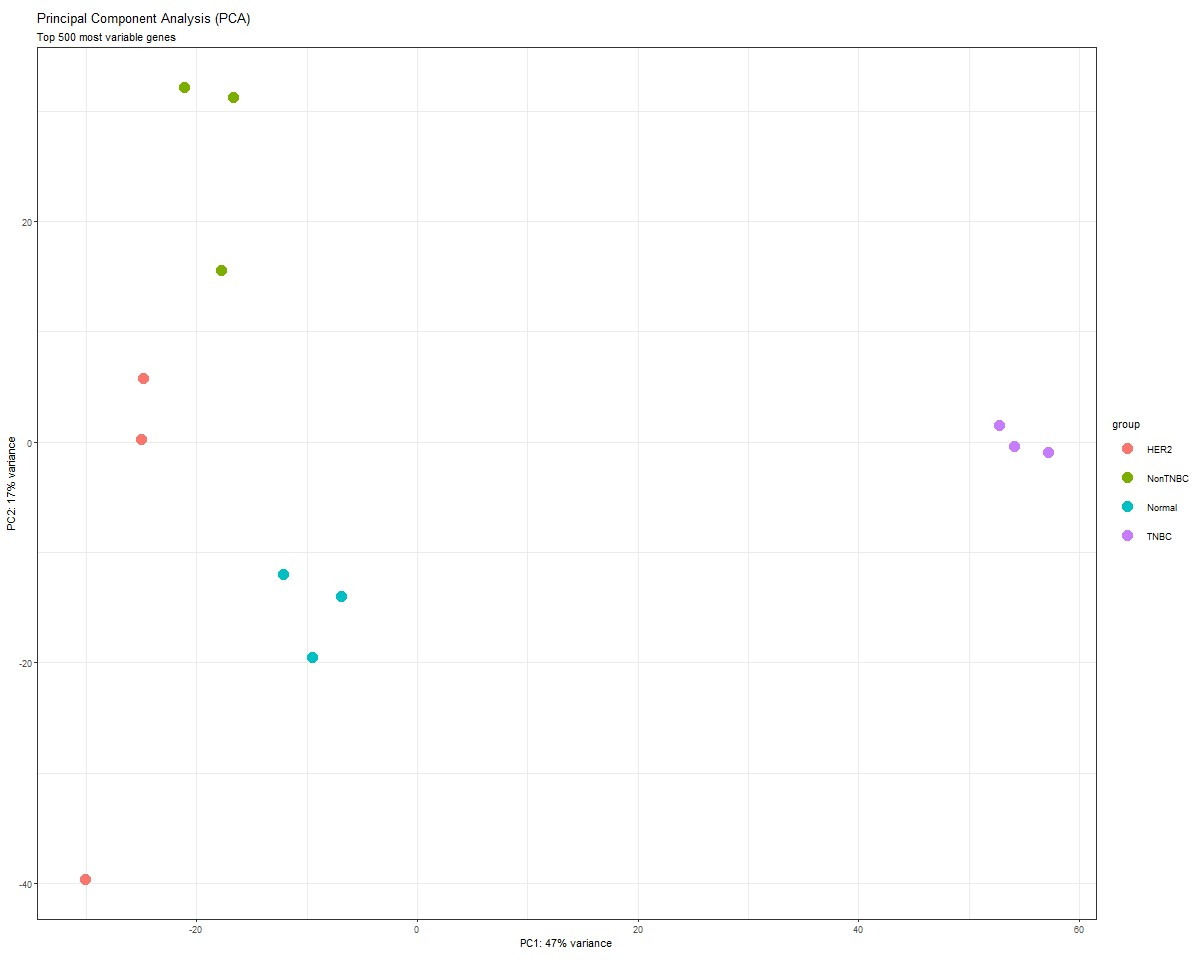
\includegraphics[width=.8\linewidth]{fig/PCA.jpg}
\caption{\label{fig:PCA}
Principle Components Analysis.}
\end{figure}

In pairwise comparison TNBC vs. NonTNBC \emph{13734} genes are differentially expressed($p_{adj} < 0.05$), 7.4\% of DE genes are up-regulated and 17\% of DE genes are down-regulated.
While in pairwise comparison HER2 vs. TNBC \emph{14514} genes are differentially expressed($p_{adj} < 0.05$).  17\% of DE genes are up-regulated and 9.2\% of DE genes are down-regulated. Vulcano Figure~\ref{fig:vulcano} shows this conclusion more visually.

\begin{figure}[t]
\centering
    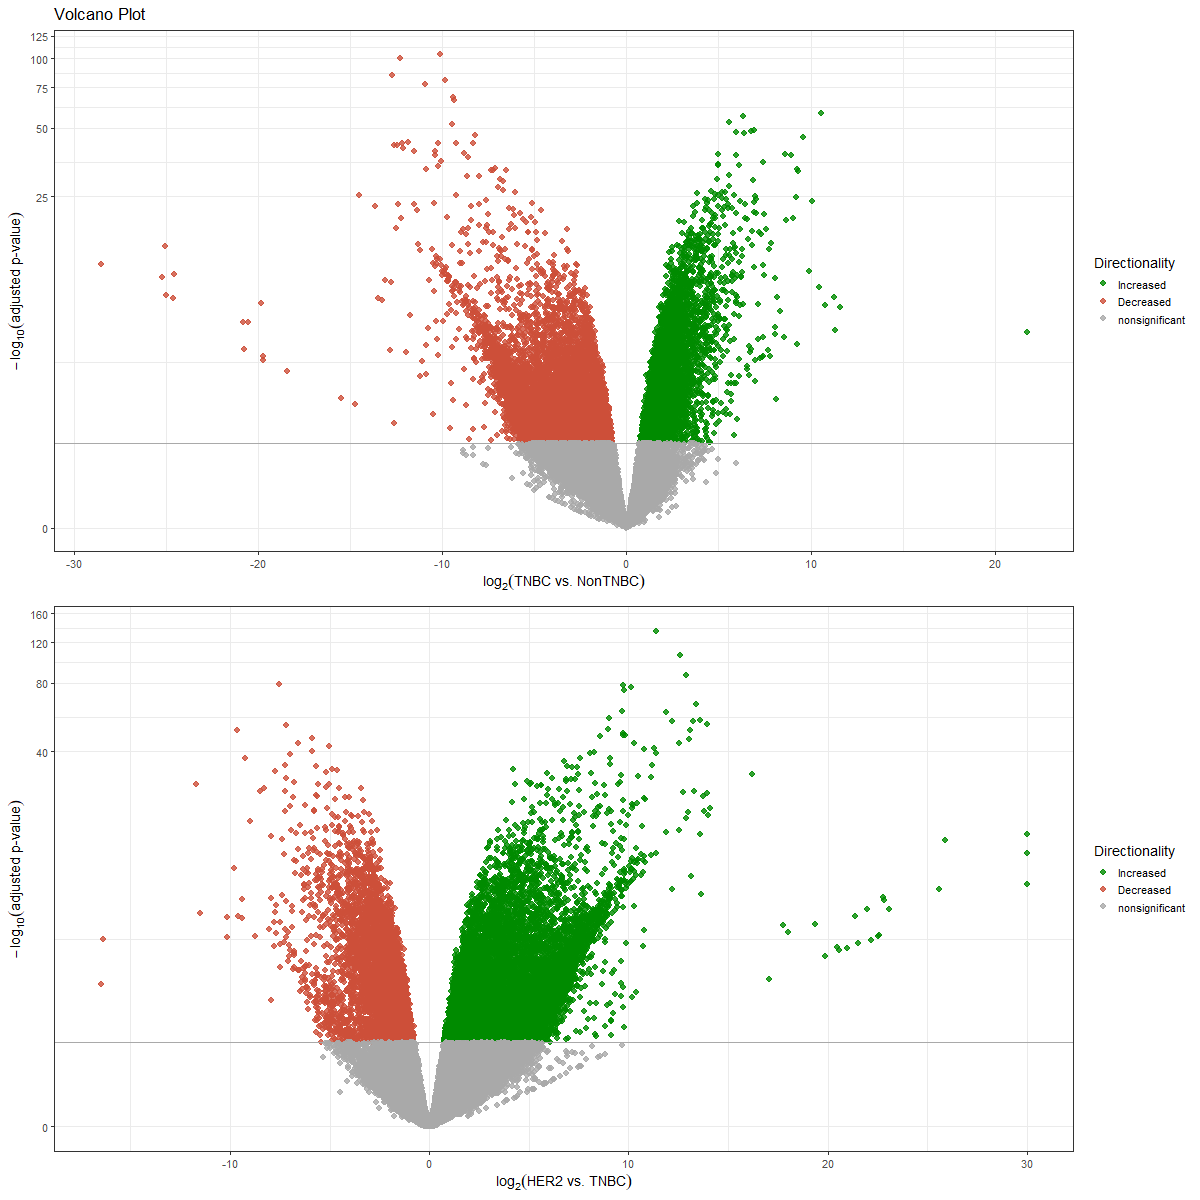
\includegraphics[width=.8\linewidth]{fig/vulcano.png}
\caption{\label{fig:vulcano}
vulcano plots TNBC vs. NonTNBC and HER2 vs. TNBC.}
\end{figure}
 
I chose SPARC and HRAS and their expression level are shown in these box plot Figure~\ref{fig:expres}. Only in TNBC human breast cancer subtype these genes results in normal condition. In other types(HER2 and NonTNBC) they cause tumors.

\begin{figure}[t]
\centering
    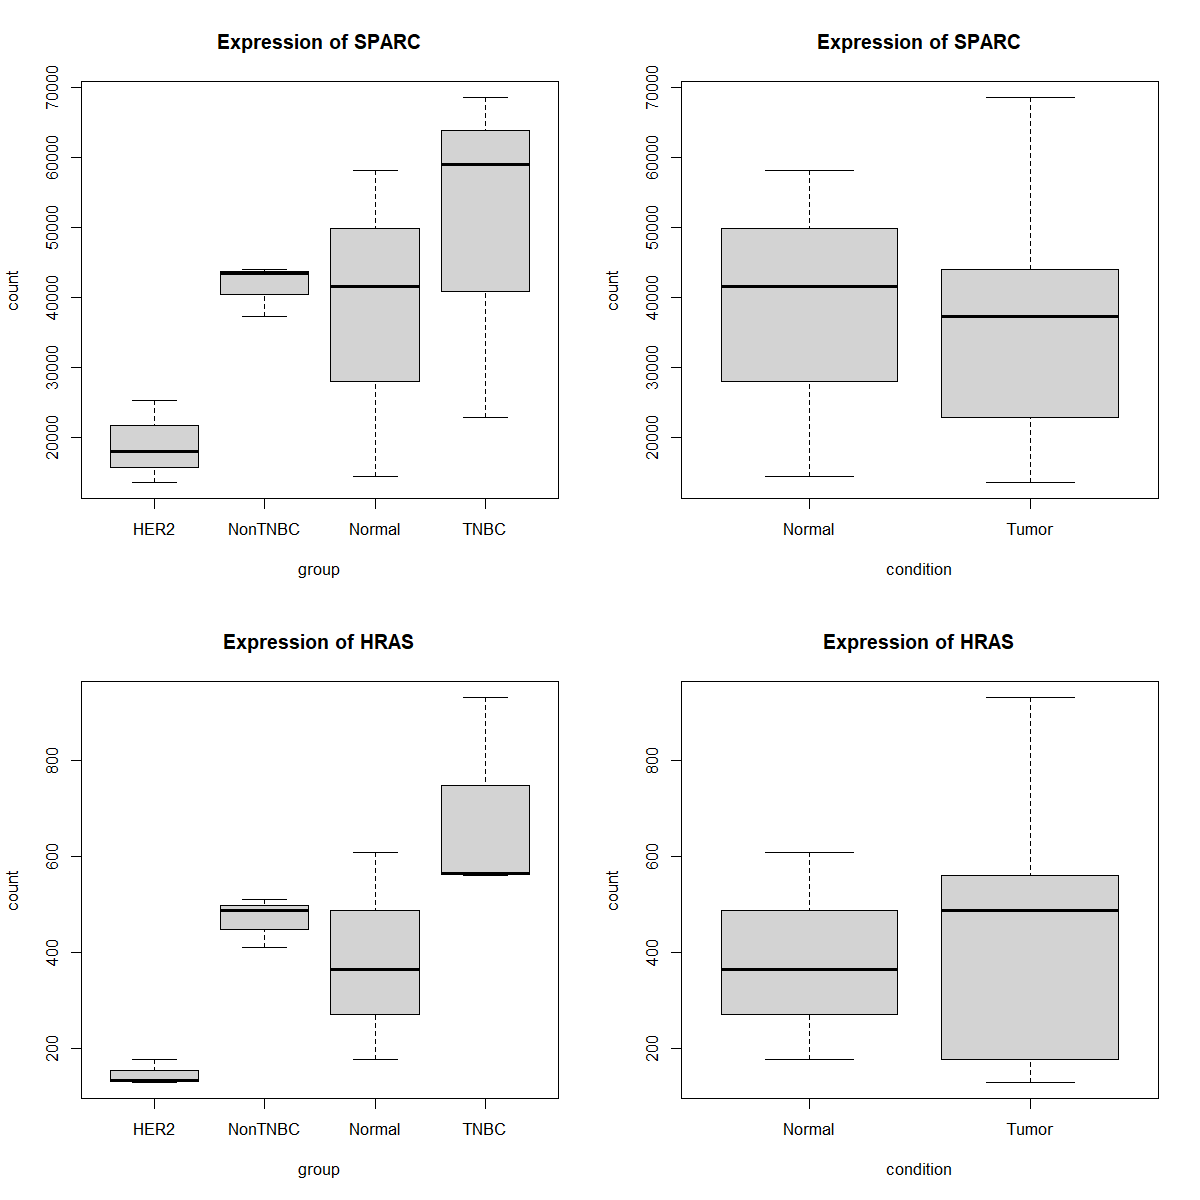
\includegraphics[width=.8\linewidth]{fig/expression.png}
\caption{\label{fig:expres}
Expression level SPARC and HRAS.}
\end{figure}

\subsection{Overrepresentation analysis}

The enrichGO function from the clusterProfiler(v.4.2.2)\cite{WU2021100141} package was used, along with the Bioconductor package org.Hs.eg.db\cite{org.Hs.eg.db}, which contains the human genome wide annotation, to  identify GO terms that include more differentially expressed genes. The \verb|dotplot| function from the enrichplot(v.1.14.1) package\cite{enrichplot} was used to show the findings.

In pairwise 2, to validate the triple negative status of our TNBC samples, the expression levels of the estrogen receptor, progesterone receptor, and HER2 were examined. Figure~\ref{fig:dotplot2} depicts the top GO keywords for the overrepresentation analysis. It shows that several of them are engaged in the immune system.

\begin{figure}[t]
\centering
\subfigure[TNBC vs. NonTNBC]{\centering
    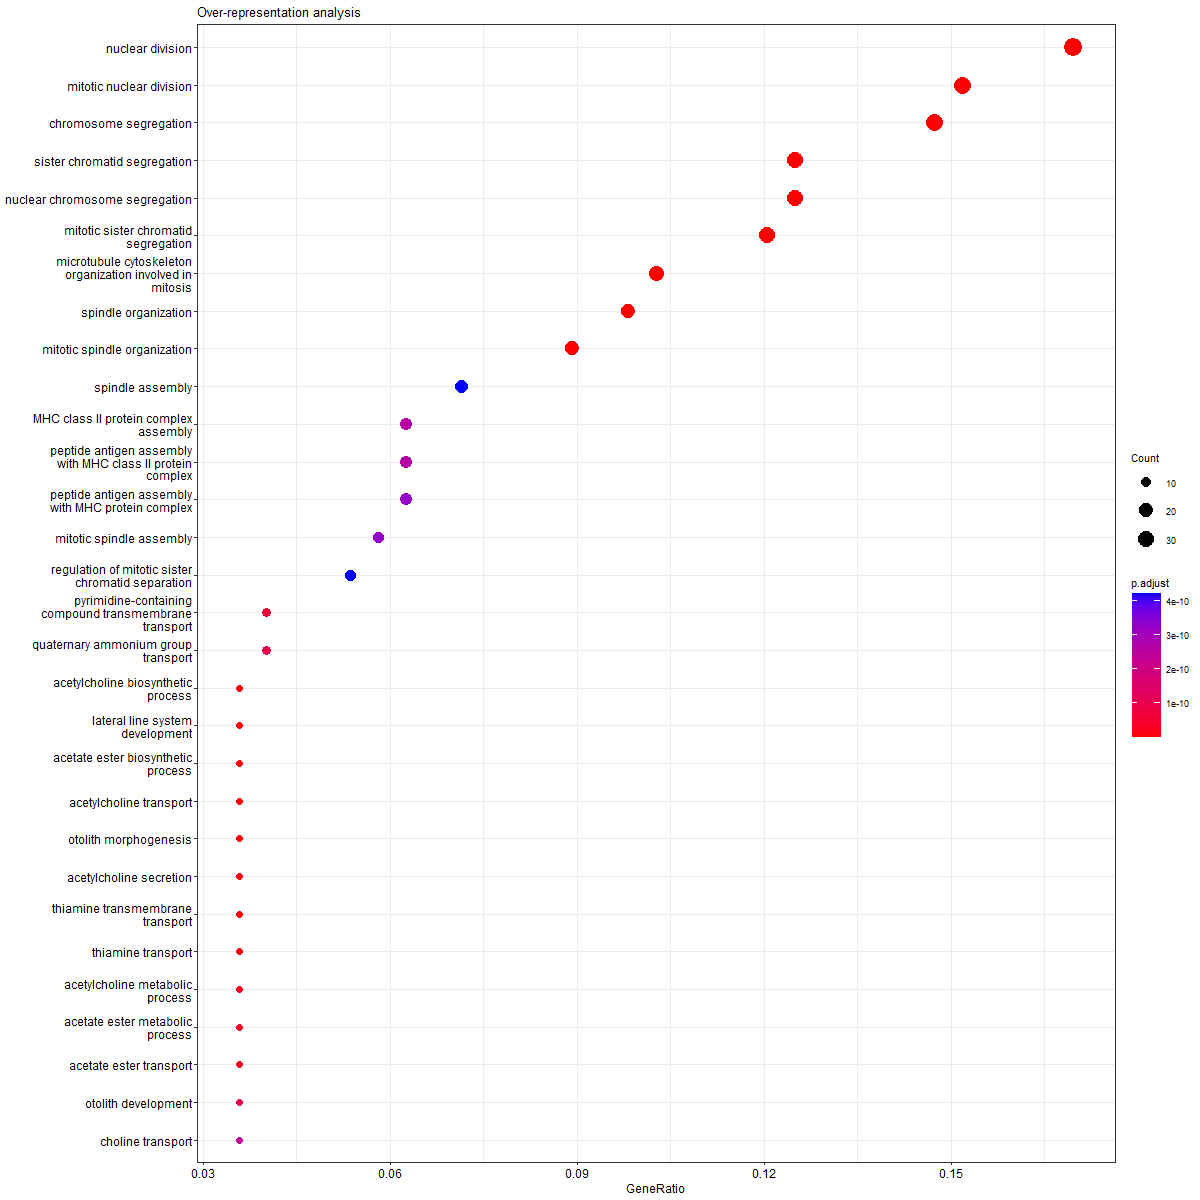
\includegraphics[width=.8\linewidth]{fig/dotplot1.png}
        \label{fig:dotplot1}}
\subfigure[HER2 vs. TNBC]{\centering
    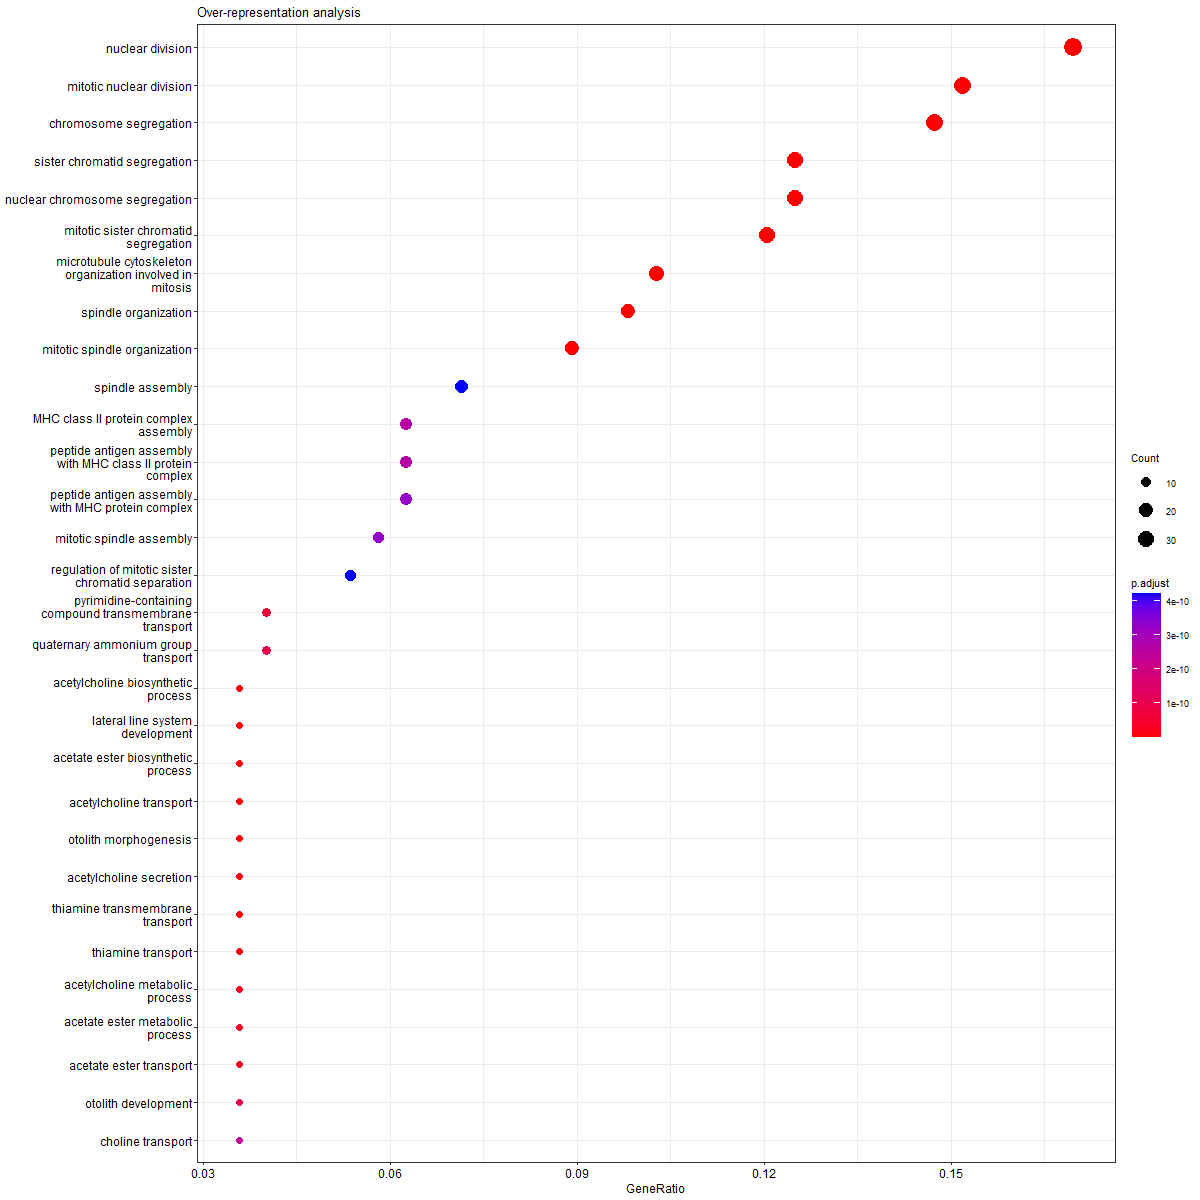
\includegraphics[width=.8\linewidth]{fig/dotplot2.png}
        \label{fig:dotplot2}}
\caption{\label{fig:dotplot}
Over-representation analysis dotplots.}
\end{figure}



\section{Discussion}

Writing bash scripts and R code to run the whole RNA-seq data analysis itself is not difficult and I think I have down a good job for reproduce my results. But coming from a computer science background interpreting the biological meaning behind the plots generated is difficult. And although I did get results in the end, the enormous number of unassigned reads caused by multimapping worries me and might have hampered the downstream analyses.

\section{Supplementary materials}

All bash and R scripts used for this project and other supplementary materials can be found
here: \url{https://github.com/kitamado/DE-analysis.}

R Packages dependencies are list at the \emph{SessionInfo} part at the end of the published RMarkdown.

Report project on Overleaf: \url{https://www.overleaf.com/read/wndtkxgggmwq}

\printbibliography


\end{document}

